Enrichment methods for continuous and categorical variables, as described in Section \ref{subsubsec:ParTIptTwo}, and Pearson product-moment correlation are applied.
Table \ref{tab:facetsValuesAttributesTable} gives a qualitative summary of all enrichments as they are presented in Appendices \ref{app:questionnaireEnrichmentTable}-\ref{app:behaviorCorrelationTable}.
Figure \ref{fig:firstEnrichmentsQuestionnaireValues} visualizes the strongest enrichments of QIs and BHVs, as well as enrichment of professional disciplines for each archetype, to give the reader an intuition of the method.
Because both enrichment and correlation methods uses \textit{distance} from archetype as the independent variable, negative slopes signify enrichment and positive slope signifies depletion.
Error bars have been omitted because they vanish due to the large sample sized, however SDs are typical in the order of a quarter of the second axis range which is not insignificant to the later interpretation of the enrichments.
All presented enrichments and correlations in Table \ref{tab:facetsValuesAttributesTable} and Figure \ref{fig:firstEnrichmentsQuestionnaireValues} are significant after Bonferroni and Benjamin-Hochberg corrections, respectively, for a significance level of 0.05.

\begin{figure}[!ht]
	\centering
	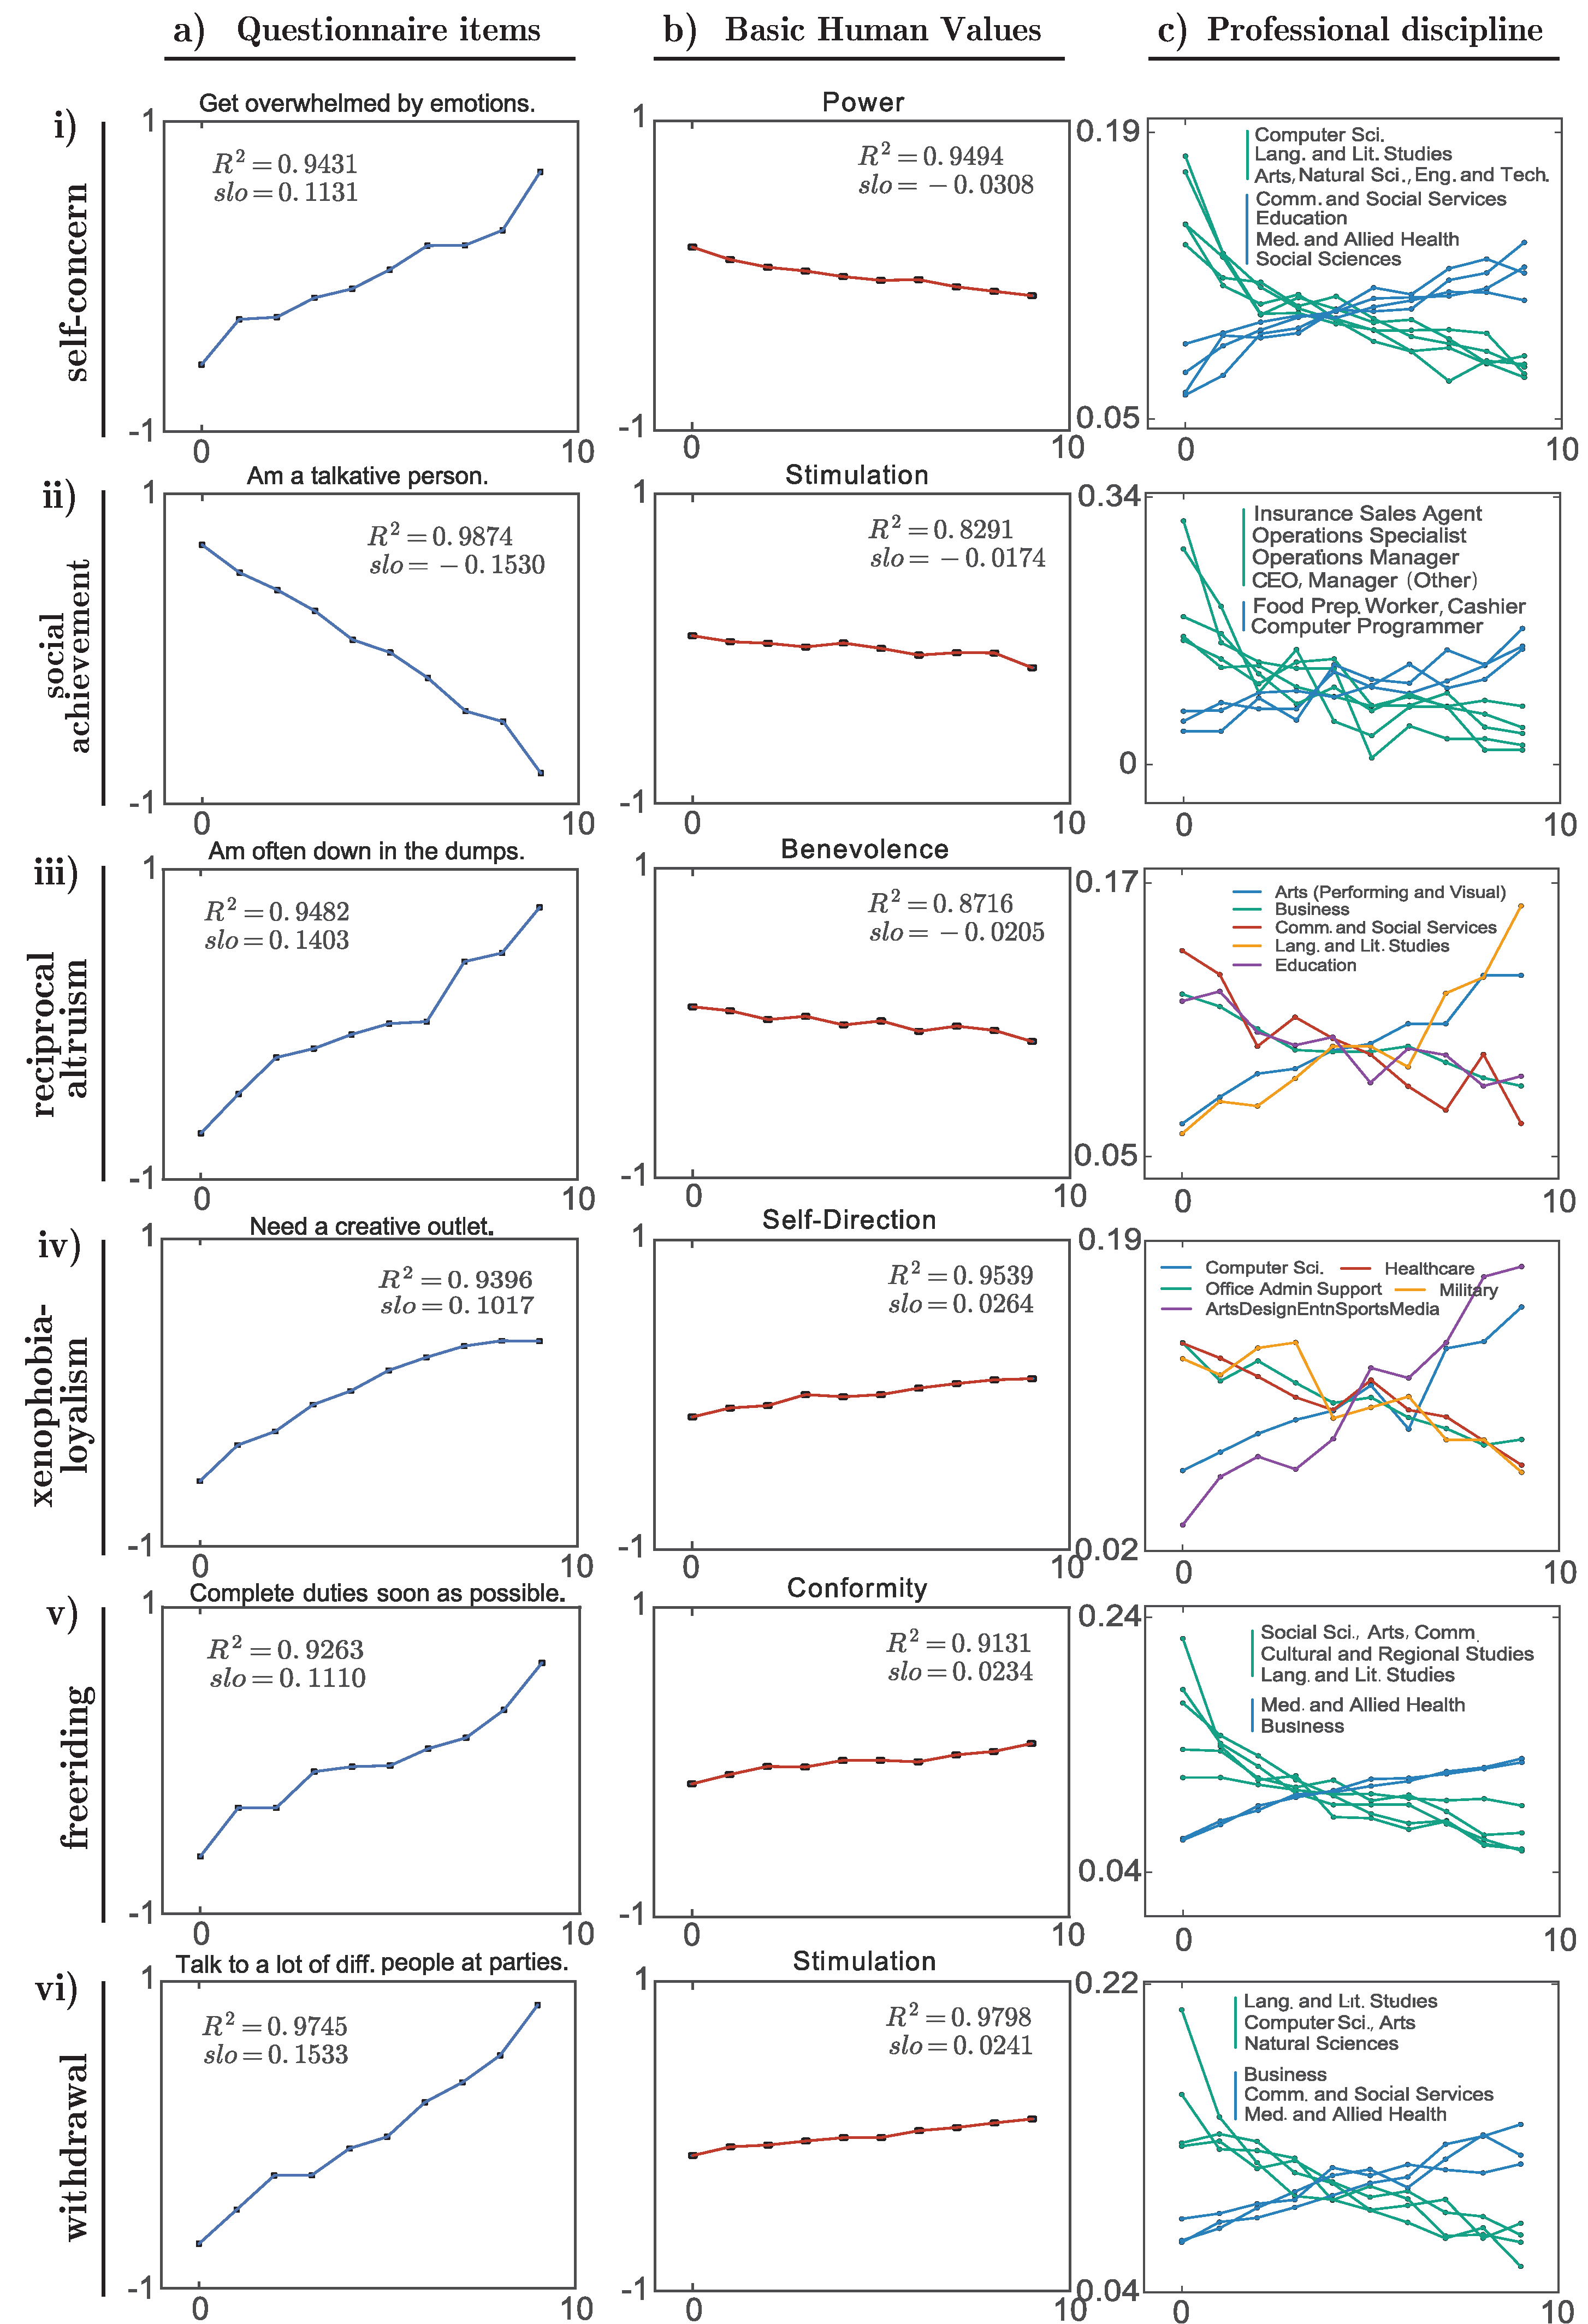
\includegraphics[width=1\textwidth]{figures/firstEnrichmentsQuestionnaireValues}
	\caption{\label{fig:firstEnrichmentsQuestionnaireValues} Enrichments for each archetype. \textbf{a-b)} are single strongest enrichments of questionnaire items ({\color{blue}blue}) and Basic Human Values ({\color{red}red}). \textbf{c)} are enrichments of professional disciplines. First axes are bin-distances from archetype and second axes for a-b) are average item response values rescaled from [1 ; 5] to [-1 ; 1] and normalized frequency for c). 'slo' is the slope of a first order approximation of the curve, so \textbf{negative slope is enrichment and positive slope is depletion}.}
\end{figure}

\begin{sidewaystable}
	% Facets and values
\newcommand{\achFac}{Emotionally stable, unsympathetic, self-concerned, exploitative, arrogant, hard to offend}
\newcommand{\hosFac}{Talkative, social, lively, moody, worrying, emotional, insecure/need reassurance, easily hurt}
\newcommand{\wilFac}{Happy, hard-working, dutiful, well-tempered, trusting, talkative, social, lively, unworried}
\newcommand{\loyFac}{Uncreative, simple-minded, ignorant, unintellectual, slow}
\newcommand{\hipFac}{Undutiful, not hard-working, disorderly, rule-breaker, don't plan ahead, unworried, calm, emotionally stable}
\newcommand{\folFac}{Not talkative, shy, antisocial, reclusive, depressed, worried, moody, irritated, panicking, emotional, lost}

\newcommand{\achVal}{Power, not benevolence, not conformity, not tradition, achievement, stimulation, hedonism}
\newcommand{\hosVal}{Stimulation, hedonism, power, achievement, universalism, security, not conformity}
\newcommand{\wilVal}{Conformity, benevolence, stimulation, achievement, tradition, security, universalism}
\newcommand{\loyVal}{Not self-direction, conformity, not stimulation, tradition, not universalism, security, not hedonism}
\newcommand{\hipVal}{Not security, not achievement, not tradition, not power, not benevolence, stimulation, hedonism}
\newcommand{\folVal}{Not stimulation, not achievement, not conformity, not power, not security, not benevolence, not hedonism, not tradition}

\newcommand{\achBeh}{-}
\newcommand{\hosBeh}{Freq. calls/texts, brief stops, goes new places, long calls, sends more texts than receives, response-rate depends on receiver, socializes at night}
\newcommand{\wilBeh}{Socializes off-campus, freq. calls/texts, goes out at night, unperiodic social pattern, brief stops, gets final word}
\newcommand{\loyBeh}{Periodic social pattern, returns calls/texts, immediate text responses, has long ongoing chats, shows up for class}
\newcommand{\hipBeh}{Short calls, unperiodic social pattern, very nocturnal, interacts with strangers, none/slow text/call responses, doesn't conclude chats}
\newcommand{\folBeh}{Doesn't meet people at campus, not nocturnal, periodic social pattern, rarely calls/texts/looks at phone, few contacts, stays home}

% Attribtues
\newcommand{\achRel}{No}
\newcommand{\achDis}{Computer sci., language and lit., arts, natural sci. eng. and tech. - not communication, edu., med. and health, social services}
\newcommand{\achJob}{Unemployed}
\newcommand{\achExe}{Yes}
\newcommand{\achSmo}{-}
\newcommand{\achAge}{Younger (0.5 years/bin), not retired}

\newcommand{\hosRel}{Yes}
\newcommand{\hosDis}{Insurance sales, operations manager/specialist, CEO - not food preparation worker, cashier, computer programmer}
\newcommand{\hosJob}{Employed}
\newcommand{\hosExe}{Yes}
\newcommand{\hosSmo}{Yes}
\newcommand{\hosAge}{Not retired}

\newcommand{\wilRel}{Yes}
\newcommand{\wilDis}{Business, education, community and social services - not arts, lang. and lit.}
\newcommand{\wilJob}{Employed, not student}
\newcommand{\wilExe}{Yes}
\newcommand{\wilSmo}{No}
\newcommand{\wilAge}{Older (-1.01 years/bin)}

\newcommand{\loyRel}{Yes}
\newcommand{\loyDis}{Healthcare, office support, military - not computer sci. and arts}
\newcommand{\loyJob}{Student, unemployed}
\newcommand{\loyExe}{-}
\newcommand{\loySmo}{No}
\newcommand{\loyAge}{Younger (0.3 years/bin)}

\newcommand{\hipRel}{No}
\newcommand{\hipDis}{Arts, cultural and regional studies, lang. and lit. studies, communication, social sci. - not business and med./health}
\newcommand{\hipJob}{Student, unemployed}
\newcommand{\hipExe}{No}
\newcommand{\hipSmo}{Yes}
\newcommand{\hipAge}{Younger (0.6 years/bin), not retired}

\newcommand{\folRel}{No}
\newcommand{\folDis}{Arts, lang. and lit., computer sci., natural sci. - not business, health-care and communication}
\newcommand{\folJob}{Unemployed}
\newcommand{\folExe}{No}
\newcommand{\folSmo}{No}
\newcommand{\folAge}{Retired}

% Row-titles
\newcommand{\achtit}{\textbf{\achiever}}
\newcommand{\hostit}{\textbf{\host}}
\newcommand{\wiltit}{\textbf{\wildcard}}
\newcommand{\loytit}{\textbf{\loyalist}}
\newcommand{\hiptit}{\textbf{\hippie}}
\newcommand{\foltit}{\textbf{\follower}}

\newcolumntype{?}{!{\vrule width 1.5pt}}
\newcommand{\mcc}[1]{\multicolumn{1}{c}{\textbf{#1}}}
\newcommand{\mccrl}[1]{\multicolumn{1}{c?}{\textbf{#1}}}

% Table
{
\footnotesize
\hspace*{-1.8cm}
\begin{tabular}{C{1.7cm}|C{2.6cm}?C{3.0cm}?C{2.7cm}|c|C{1.5cm}|c|c|C{1.5cm}?C{2.7cm}|}
\mcc{}		& \mcc{\normalsize Facets}	& \mcc{\normalsize Values}	& \multicolumn{6}{c}{ \textbf{\normalsize Demographic attributes}}												& \mcc{\normalsize Mobile behavior}	\\ \cmidrule[1pt]{2-10}
\mcc{}		& \mccrl{Highlights}		& \mccrl{Highlights}		& \mcc{Discipline}	& \mcc{Rel.ship} 	& \mcc{Job status} 	& \mcc{Exerc.} 	& \mcc{Smok.}		& \mccrl{Age} 	& \mcc{Highlights}		\\ \cline{2-10}
\achtit		& \achFac 					& \achVal 					& \achDis 			& \achRel 			& \achJob		 	& \achExe 		& \achSmo 			& \achAge 		& \achBeh				\\ \hline
\hostit 	& \hosFac 					& \hosVal 					& \hosDis 			& \hosRel 			& \hosJob		 	& \hosExe 		& \hosSmo 			& \hosAge 		& \hosBeh				\\ \hline
\wiltit 	& \wilFac 					& \wilVal 					& \wilDis 			& \wilRel 			& \wilJob		 	& \wilExe 		& \wilSmo 			& \wilAge 		& \wilBeh				\\ \hline
\loytit	 	& \loyFac 					& \loyVal 					& \loyDis 			& \loyRel 			& \loyJob		 	& \loyExe 		& \loySmo 			& \loyAge 		& \loyBeh				\\ \hline
\hiptit		& \hipFac 					& \hipVal 					& \hipDis 			& \hipRel 			& \hipJob		 	& \hipExe 		& \hipSmo 			& \hipAge 		& \hipBeh				\\ \hline
\foltit	 	& \folFac 					& \folVal 					& \folDis 			& \folRel 			& \folJob		 	& \folExe 		& \folSmo 			& \folAge 		& \folBeh				\\
\cmidrule[1pt]{2-10}
\end{tabular}
}
	\caption{\label{tab:facetsValuesAttributesTable}Summary table of the strongest significant enrichments for facets, Basic Human Values, demographic attributes and mobile behaviors for each archetype. Considering the rows one by one there are clear differences between the archetypes. Facets, values and behaviors are sorted by descending enrichment/correlation strength. The following words are shortened: sci[ence], tech[nology], eng[ineering], lit[erature], lang[uage], edu[cation] and med[icine]. '-' symbolizes no significant enrichments. Facets are single-word descriptions of longer questionnaire items (see Appendix \ref{app:questionnaireEnrichmentTable}). Demographic attributes strongly influenced by age, such as education level and marital status, are omitted due to the strong age differences between archetypes.}
\end{sidewaystable}

Two datasets provide facets, values and attributes and one provides behavior.
The SAPA-project dataset is analyzed for facets and demographic attributes.
It comprises personality test responses from a large number of Internet users, as well as demographic information such as age, gender, country, education and marital status.
This provides a unique opportunity to study how personality - or in this paradigm, distance to an archetype - links to demographic attributes.
Furthermore the property that the SAPA collection method asks respondents questions from multiple inventories is taken advantage of.
When analyzing enrichment of QIs care has been taken to avoid "circular enrichment" since distance is measured in units of BFTs and BFTs are composed of QIs.
By analyzing enrichment of QIs from the SPI inventory for individuals close to each archetype, where distance is measured using BFT values computed from the IPIP100 inventory, circularity is mitigated. 

The \textit{myPersonality} Facebook dataset is analyzed for values.
The SensibleDTU dataset is analyzed for behaviors.
Raw data is recombined into 38 behavioral indicators for 412 study participants, using an - for the purpose of this study - extended version of the behavioral feature extraction Python software \textit{bandicoot}. The indicators can be viewed in Appendix \ref{app:fullListOfExtractedFeatures}, and the implementation pipeline is presented in Section \ref{subsubsec:featureEngineering}.